\documentclass[columnsxxiv,columnsxxvii,pointsubsection]{eskdtext}

%%% eskdx
\usepackage{eskdchngsheet}		% вставка листа регистрации изменений
\usepackage{eskdfreesize}		% вставка листов нестандартного формата

%%% математика
\usepackage{amsmath,amssymb}
\usepackage{gensymb}			% знак градуса командой \degree
\usepackage{icomma}				% запятая в десятичных дробях

%%% русский язык
\usepackage[T2A]{fontenc}		% поддержка русских букв
\usepackage[utf8]{inputenc}		% кодировка ввода utf8
\usepackage[russian]{babel}		% языки: русский
% выбор русского шрифта
\IfFileExists{pscyr.sty}{%
	\usepackage{pscyr}\renewcommand{\rmdefault}{ftm}}% ftm -- TimesNewRomanPSMT (Таймс)
	{\IfFileExists{literat.sty}{\usepackage{literat}}{}}
% решение проблемы копирования текста в буфер обмена
\IfFileExists{glyphtounicode.tex}{\input glyphtounicode.tex}{}
\IfFileExists{glyphtounicode-cmr.tex}{\input glyphtounicode-cmr.tex}{}	% from pdfx package
\pdfgentounicode=1
\usepackage{cmap}				% улучшенный поиск русских слов в полученном pdf-файле

%%% списки
\usepackage{enumitem}

%%% таблицы
\usepackage{multirow}			% команда для объединения строк
\usepackage{longtable,tabu}		% сложные и длинные таблицы
\usepackage{float}				% опция [H] для точного размещения плавающих объектов
\usepackage{setspace}			% отключает полуторный интервал в окружениях table, figure, предоставляет окружение spacing{} и команды \doublespacing и др.

%%% рисование
\usepackage[europeanresistors,americaninductors]{circuitikz} % рисование электрических схем (автоподключение tikz)
\usetikzlibrary{shapes,arrows.meta,chains} % библиотеки tikz

\usepackage[ 					% гипертекстовое оглавление в PDF
	bookmarks=true, colorlinks=true, unicode=true,
	urlcolor=black,linkcolor=black, anchorcolor=black,
	citecolor=black, menucolor=black, filecolor=black,
	hypertexnames=false % можно поставить ссылку из основного документа в Приложение
	]{hyperref}
\usepackage[russian]{cleveref}	% умные ссылки

%%% микротипографика
\usepackage[final]{microtype}[2016/05/14] % улучшает представление букв и слов в строках			% пакеты
%%% обозначение
\newcommand{\org}{АБВГ}				% код разработчика
\newcommand{\num}{4362XX.XXX}		% децимальный номер изделия
\newcommand{\doc}{РЭ}				% код документа

%%% основная надпись
\ESKDtitle{Коммутатор}						% наименование изделия
\ESKDdocName{Руководство по эксплуатации}	% наименование документа
\ESKDsignature{\org.\num-01 \doc}			% обозначение документа
\ESKDauthor{}								% автор
\ESKDchecker{}								% проверил
\ESKDnormContr{}							% нормоконтролер
\ESKDapprovedBy{\hfill --- \hfill}			% утвердил
\ESKDcolumnXIfIV{ }							% согласовал
\ESKDcompany{АО << >>}						% наименование организации
\ESKDcolumnIX{\ESKDtheCompany}				% наименование организации в штампе
\ESKDcolumnXXV{\org.\num}					% обозначение документа, в котором впервые записан документ

%%% титульный лист
\newcommand{\OKPcode}{ }
\renewcommand{\ESKDtheTitleFieldIl}{\OKPcode}
\renewcommand{\ESKDtheTitleFieldX}{ }		% год
				% данные документа ЕСКД
\input{styles}				% настройки стиля
\input{setup}				% настройки документа

\graphicspath{{images/}}

\begin{document}

	\maketitle

	\newpage
	\setcounter{section}{1}
	\section{ИСПОЛЬЗОВАНИЕ ПО НАЗНАЧЕНИЮ}

	\par\vspace{6mm}\noindent ...\par\vspace{6mm}

	\setcounter{subsection}{1}
	\subsection{Монтаж изделия}

	\point
	Монтаж коммутатора должен выполняться в стандартную 19"=дюймовую монтажную стойку (шкаф) в соответствии с ГОСТ~Р~53246-2008.

	\point
	Перед началом монтажа необходимо подготовить инструмент и крепежные элементы, указанные в таблице~\ref{tab:mount-tools}.

	\renewcommand{\thetable}{\thesection.\arabic{table}}
	\renewcommand{\thefigure}{\thesection.\arabic{figure}}
	\captionsetup[table]{labelsep=emdash}
	\begin{table}[ht]
		\centering
		\captionsetup{margin=22.5mm}
		\caption{Инструмент и принадлежности для монтажа}\label{tab:mount-tools}
		\begin{tabular}{|l|l|c|l|}
			\hline
	Наименование & Назначение & Кол. & Примечание \T \\ \hline
	Отвертка крестовая PH2 & Для затяжки монтажных винтов & 1 шт. & ГОСТ 10754-80 \\ \hline
	Гайка закладная М6 (клетчатая) & Для фиксации в профиле стойки & 4 шт. & В комплекте поставки \\ \hline
	Винт М6х16 с полукруглой головкой & Для крепления кронштейнов & 4 шт. & ISO 7380 / DIN 7985 \\ \hline
	Шайба пластиковая (изоляционная) & Для защиты покрытия кронштейна & 4 шт. & В комплекте поставки \\ \hline
		\end{tabular}
	\end{table}

	\point
	Порядок проведения монтажных работ (в соответствии с рисунком~\ref{fig:mount}):

	\begin{figure}[ht]
		\centering
		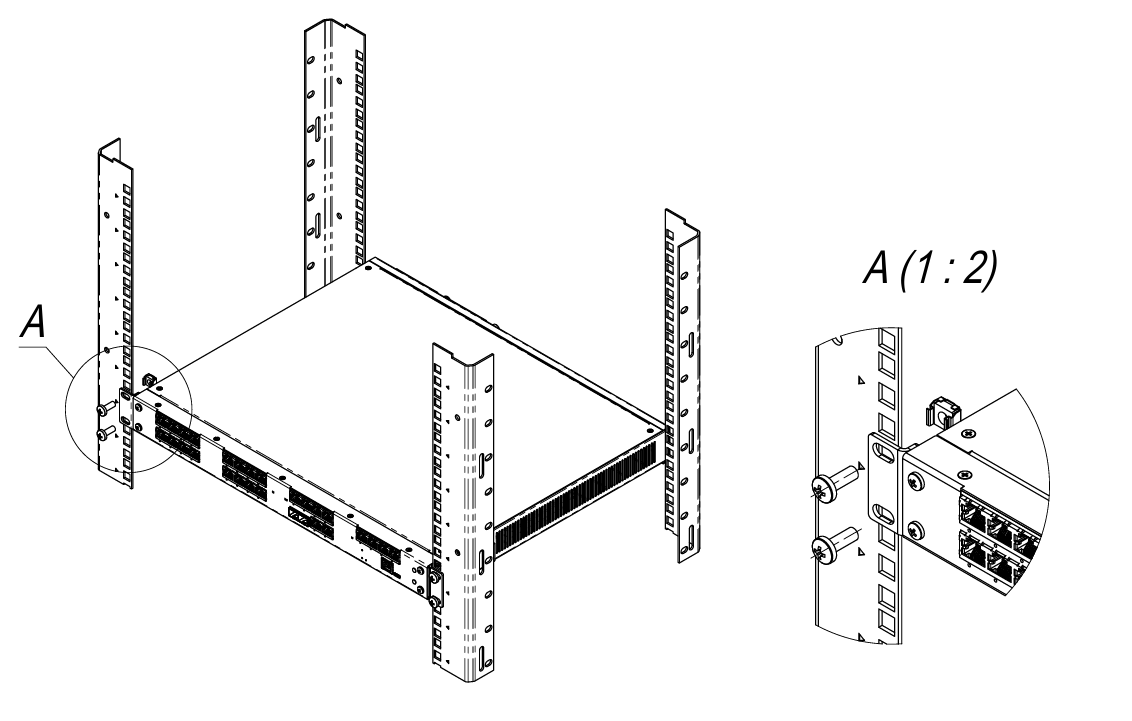
\includegraphics[width=\textwidth]{image}
		\caption{Монтаж коммутатора в монтажную стойку}
		\label{fig:mount}
	\end{figure}

	\begin{enumerate}
		\item определить требуемую высоту размещения коммутатора в монтажной стойке и разметить соответствующее количество юнитов (1U);
		\item установить четыре закладные гайки М6 в квадратные пазы вертикальных монтажных профилей стойки (по две гайки на левый и правый профили на одном уровне высоты) до защелкивания пружинных лапок зажима (см. рисунок~\ref{fig:mount}, вид~А);
		\item удерживая коммутатор, аккуратно завести его корпус в рабочее пространство стойки до совмещения пазов в монтажных кронштейнах («ушах») изделия с установленными закладными гайками;
		\item установить в совмещенные отверстия крепежные винты М6 с предварительно надетыми пластиковыми шайбами;
		\item произвести поочередную затяжку четырех винтов с помощью крестовой отвертки PH2. Усилие затяжки должно обеспечивать надежную фиксацию коммутатора без деформации монтажных кронштейнов.
	\end{enumerate}

\end{document}
